\section{Use Cases}\label{use_cases}
Aus den Anforderungen ergeben sich die in diesem Abschnitt definierten Use-Cases. Zur Übersicht dient das folgende UML Use Case Diagramm, die Details sind nachfolgend in tabellarischer Form nach \cite[S. 78-79]{pohl2010basiswissen} definiert.
\subsection{Übersicht}\label{systemfunktionalitaet}
 \begin{figure}[H]
  	\centering
    	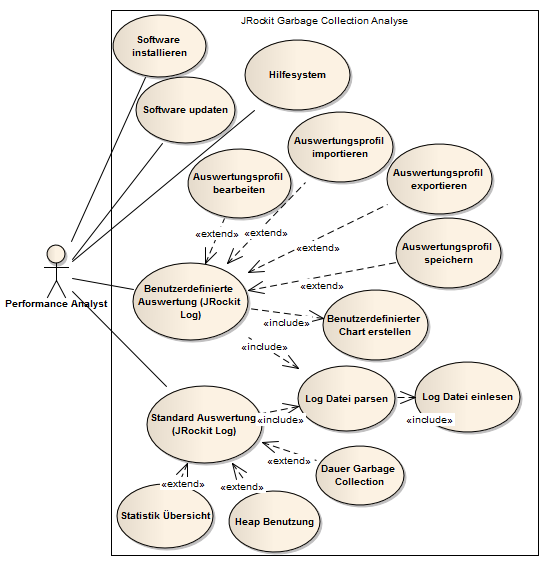
\includegraphics[width=14cm]{images/anforderungen_use-case}
        	\caption{Systemfunktionalität als Use-Case-Diagramm}
\end{figure}
\subsection{Beschreibung}
Die definierten Use Cases leiten sich aus einer Anforderung ab, welche über die Nummer referenziert ist.
\begin{longtable}{|p{4cm}|p{10.5cm}|}
  \hline
   \textbf{Abschnitt} & \textbf{Inhalt / Erläuterung} \\\hline
   Anforderung & FRQ-01\\\hline
   Bezeichner & UC-01\\\hline
   Name & Software installieren\\\hline
   Autoren & Raffael Schmid\\\hline
   Priorität & Wichtigkeit für Systemerfolg: gross\newline Technologisches Risiko: mittel\\\hline
   Kritikalität & gross\\\hline
   Verantwortlicher & Raffael Schmid\\\hline
   Kurzbeschreibung & Der Benutzer kann die Software in seiner Entwicklungsumgebung installieren.\\\hline
   Akteure & Anwender, Entwicklungsumgebung\\\hline
   Auslösendes Ereignis & Anwender möchte eine Garbage Collection Logdatei analysieren.\\\hline
   Vorbedingung & Richtige Entwicklungsumgebung ist bereits ohne Analysesoftware installiert.\\\hline
   Nachbedingung & Es sind keine Fehler aufgetreten.\\\hline
   Ergebnis & Entwicklungsumgebung ist bereit für Garbage Collection Auswertungen.\\\hline
   Hauptszenario & 
         \begin{enumerate}
		\item Anwender Startet Entwicklungsumgebung
		\item Anwender gibt Update-Seite an
		\item Anwender selektiert zu installierendes Softwarepaket
		\item Softwarepaket wird installiert	
 	\end{enumerate}
	\\\hline
   Alternativszenarien & -\\\hline
   Ausnahmeszenarien & -\\\hline
   Qualitäten & -\\\hline
\caption{Use-Case: Software installieren}
\end{longtable}

\begin{longtable}{|p{4cm}|p{10.5cm}|}
\hline
   \textbf{Abschnitt} & \textbf{Inhalt / Erläuterung} \\\hline
   Anforderung & FRQ-02\\\hline
   Bezeichner & UC-02\\\hline
   Name & Software updaten\\\hline
   Autoren & Raffael Schmid\\\hline
   Priorität & Wichtigkeit für Systemerfolg: gross\newline Technologisches Risiko: mittel\\\hline
   Kritikalität & Mittel\\\hline
   Verantwortlicher & Raffael Schmid\\\hline
   Kurzbeschreibung & Der Benutzer kann die Software updaten.\\\hline
   Akteure & Anwender, Update-Server\\\hline   
   Auslösendes Ereignis & Anwender hat die Software bereits zu einem früheren Zeitpunkt installiert. Sofern ein neues Update vorhanden ist, möchte er dieses installieren.\\\hline
   Vorbedingung & Richtige Entwicklungsumgebung und Software wurden bereits in einer früheren Version installiert.\\\hline
   Nachbedingung & Es sind keine Fehler aufgetreten.\\\hline
   Ergebnis & Entwicklungsumgebung und Analysesoftware sind auf dem neusten Stand für Garbage Collection Auswertungen.\\\hline
   Hauptszenario & 
	\begin{enumerate}
		\item Anwender Startet Entwicklungsumgebung
		\item Anwender sucht und findet Updates für die Analysesoftware
		\item Anwender selektiert eines oder mehrere dieser Softwarepakete
		\item Software wird aktualisiert
	\end{enumerate}
	\\\hline
   Alternativszenarien & -\\\hline
   Ausnahmeszenarien & -\\\hline
   Qualitäten & -\\\hline
\caption{Use-Case: Software updaten}
\end{longtable}

\begin{longtable}{|p{4cm}|p{10.5cm}|}
\hline
   \textbf{Abschnitt} & \textbf{Inhalt / Erläuterung} \\\hline
   Anforderung & FRQ-03\\\hline
   Bezeichner & UC-03\\\hline
   Name & Garbage Collection Logdatei importieren\\\hline
   Autoren & Raffael Schmid\\\hline
   Priorität & Wichtigkeit für Systemerfolg: gross\newline Technologisches Risiko: gering\\\hline
   Kritikalität & gross\\\hline
   Verantwortlicher & Raffael Schmid\\\hline
   Kurzbeschreibung & Der Benutzer importiert die sich auf dem Dateisystem befindende Logdatei.\\\hline
   Akteure & Anwender, Logdatei Importer\\\hline
   Auslösendes Ereignis & Anwender startet Garbage Collection Log Analyse\\\hline
   Vorbedingung & Logdatei befindet sich auf dem Rechner und ist in einem der unterstützten Formate. Die Software ist vollständig installiert und gestartet.\\\hline
   Nachbedingung & Es sind keine Fehler aufgetreten. \\\hline
   Ergebnis & Die Logdatei ist in der Ansicht Logdateien ersichtlich und kann von da im Analysefenster geöffnet werden.\\\hline
   Hauptszenario & 
	\begin{enumerate}
		\item Anwender öffnet Import-Wizard
		\item Anwender navigiert zum Ordner
		\item Anwender selektiert Datei(en) und importiert diese
	\end{enumerate}
	\\\hline
   Alternativszenarien & -\\\hline
   Ausnahmeszenarien & -\\\hline
   Qualitäten & -\\\hline
   Erweiterungen & UC-03.1\\\hline
\caption{Use-Case: Garbage Collection Logdatei importieren}
\end{longtable}


\begin{longtable}{|p{4cm}|p{10.5cm}|}
\hline
   \textbf{Abschnitt} & \textbf{Inhalt / Erläuterung} \\\hline
   Anforderung & FRQ-03\\\hline
   Bezeichner & UC-03.1\\\hline
   Name & Zustand Ansicht Logdateien speichern\\\hline
   Autoren & Raffael Schmid\\\hline
   Priorität & Wichtigkeit für Systemerfolg: gross\newline Technologisches Risiko: gering\\\hline
   Kritikalität & gering\\\hline
   Verantwortlicher & Raffael Schmid\\\hline
   Kurzbeschreibung & In der Ansicht Logdateien befinden sich die importierten Logdateien, der Zustand dieser Ansicht wird gespeichert und bleibt über die Zeit einer Benutzersession bestehen.\\\hline
   Akteure & Entwicklungsumgebung\\\hline
   Auslösendes Ereignis & Entwickler schliesst Entwicklungsumgebung\\\hline
   Vorbedingung & Eine oder mehrere Logdateien wurden importiert.\\\hline
   Nachbedingung & Importierte Logdateien sind gespeichert. \\\hline
   Ergebnis & Bei einem Neustart der Entwicklungsumgebung bleiben die zuvor importierten Dateien erhalten.\\\hline
   Hauptszenario & Die Information, welche Dateien importiert wurde, wird gespeichert. Beim Neustart der Software wird sie genommen um die Liste der Importierten Dateien zu initialisieren.\\\hline
   Alternativszenarien & -\\\hline
   Ausnahmeszenarien & -\\\hline
   Qualitäten & -\\\hline
\caption{Use-Case: Zustand Ansicht Logdateien speichern.}
\end{longtable}


\begin{longtable}{|p{4cm}|p{10.5cm}|}
\hline
   \textbf{Abschnitt} & \textbf{Inhalt / Erläuterung} \\\hline
   Anforderung & FRQ-04\\\hline
   Bezeichner & UC-04\\\hline
   Name & Garbage Collection Logdatei einlesen\\\hline
   Autoren & Raffael Schmid\\\hline
   Priorität & Wichtigkeit für Systemerfolg: gross\newline Technologisches Risiko: gross\\\hline
   Kritikalität & gross\\\hline
   Verantwortlicher & Raffael Schmid\\\hline
   Kurzbeschreibung & Der Benutzer kann eine sich auf seinem Rechner befindende Garbage Collection Logdatei einlesen. Die Daten befinden sich anschliessend noch im unstrukturierten Zustand, erst der Parseprozess bringt es in eine strukturierte Form (Domänenmodell).\\\hline
   Akteure & Anwender, Logdatei Importer\\\hline
   Auslösendes Ereignis & Anwender startet Auswertung\\\hline
   Vorbedingung & Logdatei wurde bereits importiert.\\\hline
   Nachbedingung & Es sind keine Fehler aufgetreten.\\\hline
   Ergebnis & Die Logdatei befindet sich im Memory und steht für das Parsen durch die spezifische Erweiterung (JRockit) zur Verfügung.\\\hline
   Hauptszenario & Anwender öffnet Logdatei im Analysefenster. Die Logdatei wird eingelesen und befindet sich für die weitere Verarbeitung durch den Parser im Arbeitsspeicher.\\\hline
   Alternativszenarien & -\\\hline
   Ausnahmeszenarien & -\\\hline
   Qualitäten & Usability (QRQ-S-04)\\\hline
\caption{Use-Case: Garbage Collection Logdatei einlesen}
\end{longtable}

\begin{longtable}{|p{4cm}|p{10.5cm}|}
\hline
   \textbf{Abschnitt} & \textbf{Inhalt / Erläuterung} \\\hline
   Anforderung & FRQ-05\\\hline
   Bezeichner & UC-05\\\hline
   Name & Garbage Collection Logdatei parsen\\\hline
   Autoren & Raffael Schmid\\\hline
   Priorität & Wichtigkeit für Systemerfolg: gross\newline Technologisches Risiko: gross\\\hline
   Kritikalität & gross\\\hline
   Verantwortlicher & Raffael Schmid\\\hline
   Kurzbeschreibung & Die sich im Arbeitsspeicher befindenden unstrukturierten Daten werden durch den Parseprozess in eine strukturierte Form gebracht (Domänenmodell). \\\hline
   Akteure & JRockit Garbage Collection Log Parser\\\hline
   Auslösendes Ereignis & Datei wurde fertig eingelesen.\\\hline
   Vorbedingung & Datei befindet sich im Arbeitsspeicher.\\\hline
   Nachbedingung & Kein Fehler ist aufgetreten.\\\hline
   Ergebnis & Domänenmodell ist fertig bereit für Abfragen darauf. \\\hline
   Hauptszenario & Jede einzelne Zeile in der Logdatei wird analysiert, die nötigen Daten werden extrahiert. Die Daten werden in ein Domänenmodell geschrieben.
	\\\hline
   Alternativszenarien & -\\\hline
   Ausnahmeszenarien & -\\\hline
   Qualitäten & Usability (QRQ-S-04), Korrektheit (QRQ-S-05)\\\hline
\caption{Use-Case: Garbage Collection Logdatei importieren}
\end{longtable}

\begin{longtable}{|p{4cm}|p{10.5cm}|}
\hline
   \textbf{Abschnitt} & \textbf{Inhalt / Erläuterung} \\\hline
   Anforderung & FRQ-06\\\hline
   Bezeichner & UC-06\\\hline
   Name & Standardauswertung anzeigen\\\hline
   Autoren & Raffael Schmid\\\hline
   Priorität & Wichtigkeit für Systemerfolg: gross\newline Technologisches Risiko: gross\\\hline
   Kritikalität & gross\\\hline
   Verantwortlicher & Raffael Schmid\\\hline
   Kurzbeschreibung & Für eine schnelle Übersicht steht eine Standard-Auswertung zur Verfügung. Diese soll eine kurze Übersicht über die Garbage Collection geben und beinhaltet zwei Charts (Heap Benutzung, Dauer Garbage Collection). \\\hline
   Akteure & Anwender, Logdatei Analyzer, Report Engine\\\hline
   Auslösendes Ereignis & Die Applikation hat die Datei fertig eingelesen und geparst.\\\hline
   Vorbedingung & Die Logdatei wurde ohne Fehler eingelesen und befindet sich im strukturierten Format im Arbeitsspeicher.\\\hline
   Nachbedingung & -\\\hline
   Ergebnis & Dem Benutzer wird ein Analyse-Screen angezeigt.\\\hline
   Hauptszenario & 
	\begin{enumerate}
		\item Applikation hat die Logdatei fertig importiert.
		\item Dem Benutzer wird ein Screen mit verschiedenen Tabs angezeigt. Auf jedem Tab wird dem Benutzer eine unterschiedliche Sicht auf die Daten gezeigt.
	\end{enumerate}
	\\\hline
   Alternativszenarien & Benutzerdefinierte Auswertung\\\hline
   Ausnahmeszenarien & -\\\hline
   Qualitäten & Korrektheit (QRQ-S-05)\\\hline
   Erweiterungen & UC-06.1, UC-06.2, UC-06.3, UC-06.4 \\\hline
\caption{Use-Case: Standardausertung anzeigen}
\end{longtable}

\begin{longtable}{|p{4cm}|p{10.5cm}|}
\hline
   \textbf{Abschnitt} & \textbf{Inhalt / Erläuterung} \\\hline
   Anforderung & FRQ-06\\\hline
   Bezeichner & UC-06.1\\\hline
   Name & Anzeige Statistik Übersicht\\\hline
   Autoren & Raffael Schmid\\\hline
   Priorität & Wichtigkeit für Systemerfolg: gross\newline Technologisches Risiko: gross\\\hline
   Kritikalität & gross\\\hline
   Verantwortlicher & Raffael Schmid\\\hline
   Kurzbeschreibung & Der Analyse-Screen wurde geöffnet, dem Benutzer zeigen sich unterschiedliche Tabs. Auf dem ersten befinden sich verschiedene statistische Auswertungen der Logdatei:
   \begin{itemize}
	\item Übersicht und Grösse der verschiedenen Bereiche auf dem Heap: Initiale Grösse, endgültige Grösse
	\item Aktivitäten des Garbage Collectors: Anzahl Young Collections, Anzahl Old Collections
	\item Anzahl Garbage Collector Events (Bsp: Wechsel der Garbage Collection Strategie, etc.)
	\item Garbage Collection Zeiten (Total, Durchschnittliche, Zeit in Old Generation Garbage Collection, Prozentuale Zeit in Old Generation Garbage Collection)
	\item Durchsatz (siehe Abschnitt \ref{gc_tuning_durchsatz})
   \end{itemize}
 \\\hline
   Qualitäten & Korrektheit (QRQ-S-05)\\\hline
\caption{Use-Case: Anzeige Statistik Übersicht}
\end{longtable}

\begin{longtable}{|p{4cm}|p{10.5cm}|}
\hline
   \textbf{Abschnitt} & \textbf{Inhalt / Erläuterung} \\\hline
   Anforderung & FRQ-06\\\hline
   Bezeichner & UC-06.2\\\hline
   Name & Anzeige Heap Benutzung\\\hline
   Autoren & Raffael Schmid\\\hline
   Priorität & Wichtigkeit für Systemerfolg: gross\newline Technologisches Risiko: gross\\\hline
   Kritikalität & gross\\\hline
   Verantwortlicher & Raffael Schmid\\\hline
   Kurzbeschreibung & Die Heap Usage (Heap Benutzung) zeigt dem Benutzer anhand einer Grafik, zu welchem Zeitpunkt wieviel Speicher des Heaps verwendet wurde. Zusätzlich werden die Zeitpunkte inklusive entsprechendem Typ (Old- / Young-Collection) der Garbage Collection angezeigt.  \\\hline
   Qualitäten & Korrektheit (QRQ-S-05)\\\hline
\caption{Use-Case: Anzeige Heap Benutzung}
\end{longtable}

\begin{longtable}{|p{4cm}|p{10.5cm}|}
\hline
   \textbf{Abschnitt} & \textbf{Inhalt / Erläuterung} \\\hline
   Anforderung & FRQ-06\\\hline
   Bezeichner & UC-06.3\\\hline
   Name & Anzeige Dauer Garbage Collection\\\hline
   Autoren & Raffael Schmid\\\hline
   Priorität & Wichtigkeit für Systemerfolg: mittel\newline Technologisches Risiko: mittel\\\hline
   Kritikalität & Mittel\\\hline
   Verantwortlicher & Raffael Schmid\\\hline
   Kurzbeschreibung & Für jede Garbage Collection ist innerhalb der Logdatei einen Eintrag mit den Informationen, wie viel Speicher von toten Objekten befreit wurde und wie lange die Collection gedauert hat. In diesem Report geht es um die Darstellung dieser Daten.\\\hline
   Qualitäten & Korrektheit (QRQ-S-05)\\\hline
\caption{Use-Case: Anzeige Dauer Garbage Collection}
\end{longtable}

\begin{longtable}{|p{4cm}|p{10.5cm}|}
\hline
   \textbf{Abschnitt} & \textbf{Inhalt / Erläuterung} \\\hline
   Anforderung & FRQ-07\\\hline
   Bezeichner & UC-07\\\hline
   Name &Profil (benutzerdefinierte Auswertung) erstellen\\\hline
   Autoren & Raffael Schmid\\\hline
   Priorität & Wichtigkeit für Systemerfolg: niedrig\newline Technologisches Risiko: niedrig\\\hline
   Kritikalität & Niedrig\\\hline
   Verantwortlicher & Raffael Schmid\\\hline
   Kurzbeschreibung & Der Benutzer kann ein eigenes Profil erstellen. Dem Profil können eigene, benutzerdefinierte Charts hinzugefügt werden (siehe UC-07.1).\\\hline
   Akteure & Anwender, Logdatei Analyzer, Report Engine\\\hline
   Auslösendes Ereignis & Die Applikation hat die Datei fertig eingelesen und geparst.\\\hline
   Vorbedingung & Die Logdatei wurde ohne Fehler eingelesen und befindet sich im strukturierten Format im Arbeitsspeicher.\\\hline
   Nachbedingung & -\\\hline
   Ergebnis & Dem Benutzer wird ein benutzerdefiniertes Analysefenster angezeigt.\\\hline
   Hauptszenario & Unabhängig vom Zyklus der Garbage Collection Analyse, kann der Benutzer ein eigenes Profil erstellen. Ein Profil besteht initial aus einem Übersichtsfenster der Garbage Collection und kann um eigene, benutzerdefinierte Charts erweitert werden.\\\hline
   Alternativszenarien & -\\\hline
   Ausnahmeszenarien & -\\\hline
   Qualitäten & Korrektheit (QRQ-S-05)\\\hline
   Erweiterungen & UC-07.1, UC-07.2, UC-07.3\\\hline

\caption{Use-Case: Profil (benutzerdefinierte Auswertung) erstellen }
\end{longtable}

\begin{longtable}{|p{4cm}|p{10.5cm}|}
\hline
   \textbf{Abschnitt} & \textbf{Inhalt / Erläuterung} \\\hline
   Anforderung & FRQ-07\\\hline
   Bezeichner & UC-07.1\\\hline
   Name & Chart definieren\\\hline
   Autoren & Raffael Schmid\\\hline
   Priorität & Wichtigkeit für Systemerfolg: niedrig\newline Technologisches Risiko: niedrig\\\hline
   Kritikalität & Niedrig\\\hline
   Verantwortlicher & Raffael Schmid\\\hline
   Kurzbeschreibung & Der Benutzer erstellt auf dem Profil ein neues Chart und definiert darauf unterschiedliche Serien\footnote{Eine Serie definiert welche Daten auf der X- respektive Y-Achse angezeigt werden sollen.}.\\\hline
   Qualitäten & -\\\hline
\caption{Use-Case: Chart definieren }
\end{longtable}

\begin{longtable}{|p{4cm}|p{10.5cm}|}
\hline
   \textbf{Abschnitt} & \textbf{Inhalt / Erläuterung} \\\hline
   Anforderung & FRQ-07\\\hline
   Bezeichner & UC-07.2\\\hline
   Name & Auswertungsprofil speichern\\\hline
   Autoren & Raffael Schmid\\\hline
   Priorität & Wichtigkeit für Systemerfolg: niedrig\newline Technologisches Risiko: niedrig\\\hline
   Kritikalität & Niedrig\\\hline
   Verantwortlicher & Raffael Schmid\\\hline
   Kurzbeschreibung & Profile können gespeichert werden und bleiben über einzelne Sitzungen bestehen, ausser der Benutzer löscht es explizit.\\\hline
   Qualitäten & -\\\hline
\caption{Use-Case: Profil speichern, löschen }
\end{longtable}

\begin{longtable}{|p{4cm}|p{10.5cm}|}
\hline
   \textbf{Abschnitt} & \textbf{Inhalt / Erläuterung} \\\hline
   Anforderung & FRQ-07\\\hline
   Bezeichner & UC-07.3\\\hline
   Name & Auswertungsprofil exportieren\\\hline
   Autoren & Raffael Schmid\\\hline
   Priorität & Wichtigkeit für Systemerfolg: niedrig\newline Technologisches Risiko: niedrig\\\hline
   Kritikalität & Niedrig\\\hline
   Verantwortlicher & Raffael Schmid\\\hline
   Kurzbeschreibung & Die vom Anwender definierten Profile können in eine Datei exportiert werden.\\\hline
   Qualitäten & -\\\hline
\caption{Use-Case: Auswertungsprofil exportieren }
\end{longtable}

\begin{longtable}{|p{4cm}|p{10.5cm}|}
\hline
   \textbf{Abschnitt} & \textbf{Inhalt / Erläuterung} \\\hline
   Anforderung & FRQ-07\\\hline
   Bezeichner & UC-07.4\\\hline
   Name & Auswertungsprofil importieren\\\hline
   Autoren & Raffael Schmid\\\hline
   Priorität & Wichtigkeit für Systemerfolg: niedrig\newline Technologisches Risiko: niedrig\\\hline
   Kritikalität & Niedrig\\\hline
   Verantwortlicher & Raffael Schmid\\\hline
   Kurzbeschreibung & Exportierte Profile können ausgetauscht und von einem anderen Benutzer in die Entwicklungsumgebung importiert werden. \\\hline
   Qualitäten & -\\\hline
\caption{Use-Case: Auswertungsprofil importieren }
\end{longtable}

\begin{longtable}{|p{4cm}|p{10.5cm}|}
\hline
   \textbf{Abschnitt} & \textbf{Inhalt / Erläuterung} \\\hline
   Anforderung & FRQ-08\\\hline
   Bezeichner & UC-8\\\hline
   Name & Hilfesystem\\\hline
   Autoren & Raffael Schmid\\\hline
   Priorität & Wichtigkeit für Systemerfolg: niedrig\newline Technologisches Risiko: mittel\\\hline
   Kritikalität & Mittel\\\hline
   Verantwortlicher & Raffael Schmid\\\hline
   Kurzbeschreibung & Dem Benutzer steht eine eine indexbasierte\footnote{Generelle Hilfe mit Informationen zur Garbage Collection,Vorgehensweise bei Performance Problemen, alternative Werkzeuge, etc.} und eine kontextsensitive\footnote{Hilfe zur aktuellen View oder Aktion des Benutzers} Hilfe zur Verfügung. \\\hline
   Akteure & Anwender\\\hline
   Auslösendes Ereignis & Anwender hat Plugin installiert, weiss nicht wie eine Analyse gestartet werden kann.\\\hline
   Vorbedingung & Entwicklungsumgebung und Software sind installiert.\\\hline
   Nachbedingung & -\\\hline
   Ergebnis & Anwender kennt Software\\\hline
   Hauptszenario &	\begin{itemize}
		\item \textbf{Indexbasierte Hilfe: } Der Benutzer kennt sich im Thema Garbage Collection und auf der Analyse-Software noch nicht aus. Er holt sich Hilfe über die indexbasierte Hilfe. 
		\item \textbf{Kontextsensitive Hilfe: } Der Benutzer befindet sich in einem Fenster oder möchte eine Aktion ausführen (Context), das Hilfesystem zeigt ihm dazu die notwendingen Informationen.
	\end{itemize}
	\\\hline
   Alternativszenarien & -\\\hline
   Ausnahmeszenarien & -\\\hline
   Qualitäten & QRQ-S-03 (Internationalisierung)\\\hline
\caption{Use-Case: Hilfesystem}
\end{longtable}

